%% eval.tex
%% $Id: eval.tex 5 2005-10-10 20:55:48Z bless $

\chapter{Evaluation}
\label{ch:Evaluation}
Die Evaluation der Ergebnisse beginnt damit, die Daten der eSense Earpods in Fenster (\textit{windows}) einzuteilen.
Auf diese Fenster werden anschließend \textit{Features} berechnet, welche die Grundlage für die Klassifizierung sind.

\section{Gibt es passende Features?}
Die Suche nach passenden Features wird mit dem Python Package \texttt{tsfresh} angegangen.
\texttt{tsfresh} berechnet automatisch Charakteristiken, sowie deren Relevanz anhand eines Zeitintervalls (\textit{Feature}) \todo{ref to website https://tsfresh.readthedocs.io}.
Diese Charakteristiken werden fortan als Features bezeichnet. \todo{wo steckt die relevanz in den tsfresh daten... }

Als Eingabe bekommt \texttt{tsfresh} die Daten der eSense Earpods, also die \textit{x, y} und \textit{z}- Achse der Gyroskop und Beschleunigungsdaten, versehen mit einem Zeitstempel. 
Anhand dieser Informationen berechnet \texttt{tsfresh} nun ($\sim$ 6000) Features für jedes Fenster.

\section{Ablauf der Evaluierung}
Im Kapitel \ref{ch:Implementierung:classification_pipeline} wurde beschrieben, wie die Features berechnet und persistiert wurden. 
Nun sind pro Studienteilnehmer für alle 3 Positionen Features berechnet worden. 
Es sind jeweils die Features für ein Fenster von 5 Sekunden und 10 Sekunden berechnet worden.
Zur Erinnerung: Jede Messung wurde in Fenster der Länge von 5, bzw. 10 Sekunden aufgeteilt, wobei jedes Fenster um eine Sekunde verschoben ist.

\subsection{Data Labeling}
Zur Klassifikation müssen die Daten bereits markiert sein, um eine Entscheidung treffen zu können. 
Beim Abspeichern der eSense Daten ist dies bereits geschehen. 
Da die Messung genau vorgibt, wann eine Person die luft anhalten soll, beziehungsweise nicht, wird diese Information mit einem \textit{Boolean} als zusätzliches Attribut vermerkt.
Da bei der Klassifikation Features anhand der eSense Daten berechnet werden, darf dieses Attribut offensichtlich nicht Teil der Featureberechnung sein.
Da nun bei einem 5 Sekunden Intervall circa 250 Einträge, bei einem 10 Sekunden Intervall circa 500 Einträge in eine Featureberechnung zusammenfließen, muss die Markierung dieses Features berechnet werden.
Ab 50\% der markierten Einträge wird das ganze Intervall als markiert gesetzt.
Dies ist eine essenzielle Entscheidung, da beim Training des Modells nun anhand dieser Markierung entschieden wird, ob ein Intervall ein Atemaussetzer repräsentiert, oder nicht.
\todo{genauer beschreiben, warum hier 50\% gewählt wurde... ich wollte bei 90\% z.B die Übergänge nicht als 0 markieren, weil dann teile der 0 markierten features eigentlich ein Atemaussetzer gewesen wäre... dann trainiert es kacke...}
Nun können die Resultate mit den Klassifikatoren verglichen werden.

\subsection{Kreuzvalidierungsverfahren}
\subsubsection{Leave One Subject Out (LOSO)}
Die Klassifikation wurde mit verschiedenen Methoden des Kreuzvalidierungsverfahren durchgeführt. 
Die erste Methode ist das \textit{Leave One Subject Out} (\textit{LOSO}) Kreuzvalidierungsverfahren. 
Hierbei wird ein Modell anhand der Daten der Studienteilnehmer trainiert, jedoch wird ein Datensatz eines Studienteilnehmers ausgelassen. 
Dieser eine Datensatz wird schließlich verwendet, um eine Vorhersage anhand der Trainingsdaten zu treffen, ohne durch interne Trainingsdaten optimiert sein zu können.
Im Folgenden wurde das LOSO Kreuzvalidierungsverfahren mit den beiden Klassifikationsalgorithmen \textit{Random Forest} und \textit{XGBoost} durchgeführt. 
Es wurde jede Person einmal ausgelassen und auf den Trainingsdatensatz angewandt, welcher diese Person nicht enthält. 
Somit entstehen 7 Resultate, von denen nun der Mittelwert gebildet wird.
Die Resultate sind in den Abbildungen \ref{evaluation:random_forest_loso:person6} und \ref{evaluation:xgboost_loso:person6} beispielhaft an Person 6 dargestellt.
Die vollständige Auflistung aller Resultate sind im Anhang zu finden. \\
Der Mittelwert aller Ergebnisse des LOSO Kreuzvalidierungsverfahrens sind im \textit{Precision} und \textit{Recall} der unterliegenden Tabelle der Beispiele bei Person 6 mit dem Mittelwert zusammengetragen worden. 
\todo{schreibe darüber, was die ergebnisse von LOSO aussagen}

Des weiteren, um mögliche Positionsabhängigkeiten zu erkennen, wurden das selbe erneut evaluiert, jedoch nur mit den einzelnen Positionsdaten der jeweiligen Person. 
In der Tabelle \ref{evaluation:loso_classification_results} sind die Resultate zu sehen.
\todo{schreibe darüber, was die ergebnisse der einzelnen personen aussagen}


%%%%%%%%%%%%%%%%%%%        RANDOM FOREST 5 sec %%%%%%%%%%%%%%%%%%%%%%%%%%%%%%%%%
\begin{figure}[H]
  \textbf{Random Forest ($w=5\si{\s}$, $d=1\si{\s}$)}
    \centering
    \begin{subfigure}{1\textwidth}
        \includegraphics[width=1\textwidth]{evaluation/loso_5sec/random_forest_loso/Random Forest (Leave one Subject out: Person 6 back).png}
        %\caption{Resultate der Person 6 auf dem Rücken liegend.}
      \end{subfigure}
      \begin{subfigure}{1\textwidth}
        \includegraphics[width=1\textwidth]{evaluation/loso_5sec/random_forest_loso/Random Forest (Leave one Subject out: Person 6 side).png}
        %\caption{Resultate der Person 6 auf der Seite liegend.}
      \end{subfigure}
      \begin{subfigure}{1\textwidth}
        \includegraphics[width=1\textwidth]{evaluation/loso_5sec/random_forest_loso/Random Forest (Leave one Subject out: Person 6 stomach).png}
        %\caption{Resultate der Person 6 auf dem Bauch liegend.}
    \end{subfigure}
    \begin{subfigure}{1\textwidth}
        \begin{center}
            \begin{tabular}{ | l | c | r | }
              \hline
               & precision & recall \\ \hline
              0 & 0.92054 & 0.74887 \\ \hline
              1 & 0.74887 & 0.66565 \\
              \hline
            \end{tabular}
        \end{center}
        \caption{Random Forest mit dem Kreuzvalidierungsverfahren. Die Tabelle zeigt den Mittelwert aller Vorhersagen der einzelnen Personen.}
        \label{implementation:app:screenshots:user_studies_information}
    \end{subfigure}
    \newline
    \vspace*{1 cm}
    \newline
    \textbf{Random Forest ($w=10\si{\s}$, $d=1\si{\s}$)}
    \begin{subfigure}{1\textwidth}
      \includegraphics[width=1\textwidth]{evaluation/loso_10sec/random_forest_loso/Random Forest (Leave one Subject out: Person 6 back).png}
      %\caption{Resultate der Person 6 auf dem Rücken liegend.}
    \end{subfigure}
    \begin{subfigure}{1\textwidth}
      \includegraphics[width=1\textwidth]{evaluation/loso_10sec/random_forest_loso/Random Forest (Leave one Subject out: Person 6 side).png}
      %\caption{Resultate der Person 6 auf der Seite liegend.}
    \end{subfigure}
    \begin{subfigure}{1\textwidth}
      \includegraphics[width=1\textwidth]{evaluation/loso_10sec/random_forest_loso/Random Forest (Leave one Subject out: Person 6 stomach).png}
      %\caption{Resultate der Person 6 auf dem Bauch liegend.}
  \end{subfigure}

  \begin{subfigure}{1\textwidth}
      \begin{center}
          \begin{tabular}{ | l | c | r | }
            \hline
             & precision & recall \\ \hline
            0 & 0.91499 & 0.76483 \\ \hline
            1 & 0.76483 & 0.67411 \\
            \hline
          \end{tabular}
      \end{center}
      \caption{Random Forest mit dem Kreuzvalidierungsverfahren (LOSO). Die Tabelle zeigt den Mittelwert aller Vorhersagen der einzelnen Personen.}
      \label{implementation:app:screenshots:user_studies_information}
  \end{subfigure}
    \caption{Das Kreuzvalidierungsverfahren (LOSO) mit dem Klassifikationsalgorithmus Random Forest. Das Modell wurde auf allen Personen, exklusive einer Person trainiert und auf alle Positionen dieser einen Person wurde eine Vorhersage getroffen. Am Beispiel hier sind die Resultate von Person 6 zu sehen. Die blauen Bereiche sind die, in denen die Luft angehalten wurde, die orangene Kurve ist die Vorhersage. ($w=$ Fenstergröße, $d=$ Verschiebung der Fenster)}
\label{evaluation:random_forest_loso:person6}
\end{figure}

%%%%%%%%%%%%%%%%%%%        XG BOOST 5 sec %%%%%%%%%%%%%%%%%%%%%%%%%%%%%%%%%

\begin{figure}[H]
  \textbf{XG Boost ($w=5\si{\s}$, $d=1\si{\s}$)}
    \centering
    \begin{subfigure}{1\textwidth}
        \includegraphics[width=1\textwidth]{evaluation/loso_5sec/xg_boost_loso/XG Boost (Leave one Subject out: Person 6 back).png}
        %\caption{Resultate der Person 6 auf dem Rücken liegend.}
      \end{subfigure}
      \begin{subfigure}{1\textwidth}
        \includegraphics[width=1\textwidth]{evaluation/loso_5sec/xg_boost_loso/XG Boost (Leave one Subject out: Person 6 side).png}
        %\caption{Resultate der Person 6 auf der Seite liegend.}
      \end{subfigure}
      \begin{subfigure}{1\textwidth}
        \includegraphics[width=1\textwidth]{evaluation/loso_5sec/xg_boost_loso/XG Boost (Leave one Subject out: Person 6 stomach).png}
        %\caption{Resultate der Person 6 auf dem Bauch liegend.}
    \end{subfigure}

    \begin{subfigure}{1\textwidth}
        \begin{center}
            \begin{tabular}{ | l | c | r | }
              \hline
               & precision & recall \\ \hline
              0 & 0.93269 & 0.69694 \\ \hline
              1 & 0.69694 & 0.72791 \\
              \hline
            \end{tabular}
        \end{center}
        \caption{XGBoost mit dem Kreuzvalidierungsverfahren (LOSO). Die Tabelle zeigt den Mittelwert aller Vorhersagen der einzelnen Personen.}
        \label{implementation:app:screenshots:user_studies_information}
    \end{subfigure}
    \newline
    \vspace*{1 cm}
    \newline
    \textbf{XG Boost ($w=10\si{\s}$, $d=1\si{\s}$)}
    \begin{subfigure}{1\textwidth}
      \includegraphics[width=1\textwidth]{evaluation/loso_10sec/xg_boost_loso/XG Boost (Leave one Subject out: Person 6 back).png}
      %\caption{Klassifikationsresultate der Person 6. Die Messung wurde auf dem Rücken liegend durchgeführt.}
    \end{subfigure}
    \begin{subfigure}{1\textwidth}
      \includegraphics[width=1\textwidth]{evaluation/loso_10sec/xg_boost_loso/XG Boost (Leave one Subject out: Person 6 side).png}
      %\caption{Klassifikationsresultate der Person 6. Die Messung wurde auf der Seite liegend durchgeführt.}
    \end{subfigure}
    \begin{subfigure}{1\textwidth}
      \includegraphics[width=1\textwidth]{evaluation/loso_10sec/xg_boost_loso/XG Boost (Leave one Subject out: Person 6 stomach).png}
      %\caption{Klassifikationsresultate der Person 6. Die Messung wurde auf dem Bauch liegend durchgeführt.}
  \end{subfigure}

  \begin{subfigure}{1\textwidth}
      \begin{center}
          \begin{tabular}{ | l | c | r | }
            \hline
             & precision & recall \\ \hline
            0 & 0.93186 & 0.74072 \\ \hline
            1 & 0.74072 & 0.74767 \\
            \hline
          \end{tabular}
      \end{center}
      \caption{XGBoost mit dem Kreuzvalidierungsverfahren (LOSO). Die Tabelle zeigt den Mittelwert aller Vorhersagen der einzelnen Personen.}
      \label{implementation:app:screenshots:user_studies_information}
  \end{subfigure}
    \caption{Das Kreuzvalidierungsverfahren (LOSO) mit dem Klassifikationsalgorithmus XG Boost. Das Modell wurde auf allen Personen, exklusive einer Person trainiert und auf alle Positionen dieser einen Person wurde eine Vorhersage getroffen. Am Beispiel hier sind die Resultate von Person 6 zu sehen. Die blauen Bereiche sind die, in denen die Luft angehalten wurde, die orangene Kurve ist die Vorhersage. ($w=$ Fenstergröße, $d=$ Verschiebung der Fenster)}
\label{evaluation:xgboost_loso:person6}
\end{figure}

%%%%%%%%%%%%%%%%%%%        Position based results  5 sec %%%%%%%%%%%%%%%%%%%%%%%%%%%%%%%%%
\begin{table}
\begin{tabular}{cc}    
    \begin{minipage}{.33\linewidth}
        \begin{center}
            \begin{tabular}{ | l | c | r | }
              \hline
               & precision & recall \\ \hline
              0 & 0.89921 & 0.71875 \\ \hline
              1 & 0.71875 & 0.57238 \\
              \hline
            \end{tabular}
            \smallskip
            \\ Random Forest (only side, \textit{window: 5s})
        \end{center}
        %\label{evaluation:5s:random_forest_loso_side}
    \end{minipage}

    \begin{minipage}{.33\linewidth}
        \begin{center}
            \begin{tabular}{ | l | c | r | }
              \hline
               & precision & recall \\ \hline
              0 & 0.89094 & 0.82538 \\ \hline
              1 & 0.82538 & 0.44796 \\
              \hline
            \end{tabular}
            \smallskip
            \\ Random Forest (only back, \textit{window: 5s})
        \end{center}
        %\label{evaluation:5s:random_forest_loso_back}
    \end{minipage}

    \begin{minipage}{0.33\textwidth}
        \begin{center}
            \begin{tabular}{ | l | c | r | }
              \hline
               & precision & recall \\ \hline
              0 & 0.92421 & 0.72336 \\ \hline
              1 & 0.723369 & 0.65753 \\
              \hline
            \end{tabular}
            \smallskip
            \\ Random Forest (only stomach, \textit{window: 5s})
        \end{center}
        %\label{evaluation:5s:random_forest_loso_stomach}
    \end{minipage}
\end{tabular}
\newline
\vspace*{5mm}
\newline
\begin{tabular}{cc}
    \begin{minipage}{0.33\textwidth}
        \begin{center}
            \begin{tabular}{ | l | c | r | }
              \hline
               & precision & recall \\ \hline
              0 & 0.91483 & 0.6697 \\ \hline
              1 & 0.66979 & 0.6116 \\
              \hline
            \end{tabular}
            \smallskip
            \\ XG Boost (only side, \textit{window: 5s})
        \end{center}
        %\label{evaluation:5s:xg_boost_loso_side}
    \end{minipage}

    \begin{minipage}{0.33\textwidth}
        \begin{center}
            \begin{tabular}{ | l | c | r | }
              \hline
               & precision & recall \\ \hline
              0 & 0.89937 & 0.75145 \\ \hline
              1 & 0.75145 & 0.54108 \\
              \hline
            \end{tabular}
            \smallskip
            \\ XG Boost (only back, \textit{window: 5s})
        \end{center}
        %\label{evaluation:5s:xg_boost_loso_back}
    \end{minipage}

    \begin{minipage}{0.33\textwidth}
        \begin{center}
            \begin{tabular}{ | l | c | r | }
              \hline
               & precision & recall \\ \hline
              0 & 0.94418 & 0.70734 \\ \hline
              1 & 0.70734 & 0.71763 \\
              \hline
            \end{tabular}
            \smallskip 
            \\ XG Boost (only stomach, \textit{window: 5s})
        \end{center}
        %\label{evaluation:5s:xg_boost_loso_stomach}
    \end{minipage}
\end{tabular}
\newline
\vspace*{5mm}
\newline
%%%%%%%%%%%%%%%%%%%        Position based results  10 sec %%%%%%%%%%%%%%%%%%%%%%%%%%%%%%%%%
  \begin{tabular}{cc}    
      \begin{minipage}{.33\linewidth}
          \begin{center}
              \begin{tabular}{ | l | c | r | }
                \hline
                 & precision & recall \\ \hline
                0 & 0.89103 & 0.79443 \\ \hline
                1 & 0.79443 & 0.53429 \\
                \hline
              \end{tabular}
              \smallskip
              \\ Random Forest (only side, \textit{window: 10s})
          \end{center}
          %\label{evaluation:5s:random_forest_loso_side}
      \end{minipage}
  
      \begin{minipage}{.33\linewidth}
          \begin{center}
              \begin{tabular}{ | l | c | r | }
                \hline
                 & precision & recall \\ \hline
                0 & 0.88568 & 0.79427 \\ \hline
                1 & 0.79427 & 0.52266 \\
                \hline
              \end{tabular}
              \smallskip
              \\ Random Forest (only back, \textit{window: 10s})
          \end{center}
          %\label{evaluation:5s:random_forest_loso_back}
      \end{minipage}
 
      \begin{minipage}{0.33\textwidth}
          \begin{center}
              \begin{tabular}{ | l | c | r | }
                \hline
                 & precision & recall \\ \hline
                0 & 0.94411 & 0.71447 \\ \hline
                1 & 0.71447 & 0.73037 \\
                \hline
              \end{tabular}
              \smallskip
              \\ Random Forest (only stomach, \textit{window: 10s})
          \end{center}
          %\label{evaluation:5s:random_forest_loso_stomach}
      \end{minipage}
  \end{tabular}
  \newline
  \vspace*{5mm}
  \newline
  \begin{tabular}{cc}
      \begin{minipage}{0.33\textwidth}
          \begin{center}
              \begin{tabular}{ | l | c | r | }
                \hline
                 & precision & recall \\ \hline
                0 & 0.90497 & 0.78440 \\ \hline
                1 & 0.78440 & 0.60745 \\
                \hline
              \end{tabular}
              \smallskip
              \\ XG Boost (only side, \textit{window: 10s})
          \end{center}
          %\label{evaluation:5s:xg_boost_loso_side}
      \end{minipage}

      \begin{minipage}{0.33\textwidth}
          \begin{center}
              \begin{tabular}{ | l | c | r | }
                \hline
                 & precision & recall \\ \hline
                0 & 0.90300 & 0.75056 \\ \hline
                1 & 0.75056 & 0.57973 \\
                \hline
              \end{tabular}
              \smallskip
              \\ XG Boost (only back, \textit{window: 10s})
          \end{center}
          %\label{evaluation:5s:xg_boost_loso_back}
      \end{minipage}
  
      \begin{minipage}{0.33\textwidth}
          \begin{center}
              \begin{tabular}{ | l | c | r | }
                \hline
                 & precision & recall \\ \hline
                0 & 0.93783 & 0.71278 \\ \hline
                1 & 0.71278 & 0.72075 \\
                \hline
              \end{tabular}
              \smallskip 
              \\ XG Boost (only stomach, \textit{window: 10s})
          \end{center}
          %\label{evaluation:5s:xg_boost_loso_stomach}
      \end{minipage}
  \end{tabular}
  \caption{Klassifikationsergebnisse mit dem Kreuzvalidierungsverfahren bei einer Fenstergröße von 5, bzw. 10 Sekunden, welche um 1 Sekunde verschoben wurden. Es wurde immer eine Person aus dem Trainieren des Modells ausgelassen und auf diese Person wurde anschließend eine Vorhersage getroffen. Jede Person wurde einmel in dem Modell außen vorgelassen und auf dieses Modell vorhergesagt. Das zu sehende Resultat ist der Mittelwert aller Resultate des Kreuzvalidierungsverfahrens der einzelnen Positionen der Position.}
  \label{evaluation:loso_classification_results}
  \end{table}


Jede Klassifikation ergab ein Resultat, welches durch einzelne Features entschieden wurde. 
Um einen kleinen Überblick zu bekommen, welche Features entscheidend für die Evaluation waren, sind nun einige aufgelistet.
\begin{itemize}
    \item gyroZ partial autocorrelation
    \item gytoX fft coefficient
    \item gyroX agg autocorrelation
    \item accY autocorrelation
    \item gyroY change quantiles 
    \item gyroZ fft coefficient
\end{itemize}
Diese Features wurden mittels \texttt{tsfresh} berechnet und waren bei der Klassifikation des Kreuzvalidierungsverfahrens entscheidened.

\subsubsection{Within Subject}
Als zweites Kreuzvalidierungsverfahren wird \textit{Within Subject} angewandt.
Hier wird versucht, alle Personen mit der Methode \texttt{test\_train\_split} die ganzen Daten in Trainingsdaten und Testdaten aufzuteilen.
Hier wird eine Aufteilung von 70\% für die Trainingsdaten und 30\% für die Testdaten gewählt. 
Daraus ergibt sich ein \textit{score}, welcher \todo{was gibt mit der score}
Die Resultate sind in Abbildung \ref{evaluation:within_subject_results} zu sehen.
\todo{daraus erkennt man folgendes:}

\begin{table}
  \begin{tabular}{cc}
    \begin{minipage}{1\textwidth}
      \begin{center}
          \begin{tabular}{ | l | c | c | c | c | c | }
            \hline
            \textbf{Verfahren} & \textbf{Positionen} & \textbf{Score} & \textbf{Score} & \textbf{Score} & \textbf{Score} \\ 
            & & \textbf{$w=5\si{\s}$} & \textbf{$w=5\si{\s}$} & \textbf{$w=10\si{\s}$} & \textbf{$w=10\si{\s}$} \\
            & & \textbf{$d=1\si{\s}$} & \textbf{$d=5\si{\s}$} & \textbf{$d=1\si{\s}$} & \textbf{$d=10\si{\s}$} \\ \hline
            Random Forest & Alle &  0.87081 & 0.73988 & 0.89300 & 0.71428 \\ 
             & Rücken & 0.85517 & 0.66666 & 0.93333 & 0.57142 \\
             & Seite  & 0.85763 & 0.72413 & 0.89523 & 0.75 \\
             & Bauch  & 0.89619 & 0.84745 & 0.92332 & 0.65714 \\ \hline
            XG Boost  & Alle & 0.88004 & 0.69942 & 0.91737 & 0.76190 \\ 
             & Rücken & 0.88965 & 0.66666 & 0.95238 & 0.62857 \\
             & Seite  & 0.90277 & 0.77586 & 0.92380 & 0.47222 \\
             & Bauch  & 0.90311 & 0.74576 & 0.94888 & 0.62857 \\ \hline
            SVM & Alle& 0.54209 & 0.47976 & 0.65360 & 0.41904 \\ 
             & Rücken & 0.59655 & 0.66666 & 0.71746 & 0.45714 \\
             & Seite  & 0.56597 & 0.37931 & 0.62539 & 0.5 \\
             & Bauch  & 0.61245 & 0.40677 & 0.67412 & 0.4 \\
            \hline
          \end{tabular}
      \end{center}
    \end{minipage}
  \end{tabular}
  \caption{Ergebnisse des Kreuzvalidierungsverfahrens innerhalb eines Subjects mit einer Aufteilung von 70\% Trainings- und 30\% Testdaten. Alle Personen der Nutzerstudie wurden verwendet. $w$ steht für die Fenstergröße, $d$ für die Verschiebung der aneinanderfolgenden Fenster.}
  \label{evaluation:within_subject_results}
\end{table}

die ergebnisse sind in abb zu finden... 
evaluation der ergebnisse

Was bieten die verfahren, wie macht das sinn, dass sinnvolle ergebnisse herauskommen...

WelcheVor-undNachteilekönnendieseVerfahrenbieten?

\section{Erkenntnisse}
\todo{ich habe gelernt}
\begin{itemize}
    \item auswertungsdaten: Auf dem rücken liegende ddaten sind am vielversprechendsten
    \item die atempausen können einigermaßen klassifiziert werden
    \item rauschen entfernen bringt nix vermutlich wegen tsfresh, da es das schon macht, also es kommen
    \item 
\end{itemize}

gibt earables, die blutsauerstoff und puls mittracken können
plus grafik telegram tobi